\section{Informationstheorie}
\subsection{Grundlagen}\script{203}\label{entropie}~\\
\textbf{Entropie} $H(X)$ (in [bit/Symbol]) ist der statistisch gemittelte Informationsgehalt. Ist die Quelle (DMS) gedächnisfrei, entspricht dies gerade dem Erwartungswert:
\[
H(X) = E[I(x_i)] = \sum_{i}P(X_i)I(X_i) = -\sum_{i}P(X_i)\log_2P(X_i)
\]
Die \textbf{maximale Entropie} $H_{max}(X) = \log_2 m$ was im binären Fall $m=2$ genau $1$ ergibt. Die Entropie kann bei unabhängigen Quellen summiert werden.~\\~\\

\textbf{Informationsgehalt I}
\[
I(X_i) = -\log_2P(x_i)
\]

\textbf{Redundanz}
\[
R = H_{max} - H(X)
\]

\textbf{Informationsrate}
Die Symbolrate/Bitrate $r$ in [Symbole/s] ergeben die Informationsrate $R_I$
\[
R_I = r\cdot H(X)
\]

\subsection{Discrete Memoryless Channel - DMC}
Ein Kanal bildet Eingangssignal $x_i$ auf ein Ausgangssymbol $y_k$ ab. Diese Abbildung erfolgt mit einer Wahrscheinlichkeit $P(y_k | x_i)$.
Die Kanalmatrix gibt die Wahrscheinlichkeit wieder, dass aus $x_i$ ein $y_k$ wird. Es gilt für alle Matrizen: $\mathbf{P}(Y) = \mathbf{P}(X) \cdot \mathbf{P}(Y|X)$
\[
P(Y|X) = \begin{pmatrix}
	P(y_1|x_1) & \dots & P(y_n|x_n) \\
	\vdots & \ddots & \vdots \\
	P(y_1|x_m) & \dots & P(y_n,x_m)
\end{pmatrix}
\]
Die Verbundmatrix gibt ein zusätzliches gewicht mit der Wahrscheinlichkeit $P(x_i)$

\noindent\textbf{Beispiel}: Die Kanalmatrix mit $m=3$ möglichen Eingängen und $n=5$ Ausgängen.
\[
P(Y|X) = \begin{pmatrix}
	\frac{3}{4} & \frac{1}{4} & 0 &0 &0 \\
	0 &0 &\frac{1}{3} & \frac{2}{3} &0 \\
	0 & 0 & 0 &0 &1 \\
\end{pmatrix}
\]
Das \textbf{Kanaldiagramm} sieht mit $P$ folgendermassen aus.
\begin{center}
	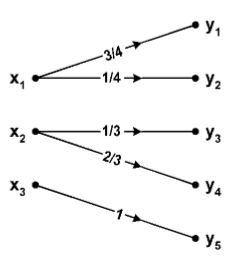
\includegraphics[width=0.3\columnwidth]{Images/kanaldiagramm}
\end{center}
Weitere wichtige Modelle sind im \script{204}

\subsubsection{Kanalkapazität}
Die Kanalkapazität pro Symbol $C_s$ berechnet sich für ein \textbf{binären symmetrischen Kanal} mit. Weiter Kanäle im \script{207}
\[
C_s = 1 + p_e\cdot \log_2p_e + (1 - p_e)\cdot\log_2(1- p_e)
\]

Allgemein für ein AWGN-Rauschkanal kann abgeschätzt werden mit:
\[
C_s = \frac{1}{2}\cdot \log_2\left(1 + \frac{S}{N}\right)
\]
Dabei ist $\frac{S}{N}$ die Single-to-noise Ratio im linearen Verhältnis (nicht in dB). Für $C_{bps} = 2\cdot B \cdot C_s$ mit Bandbreite nach Shannon-Hartly-Gesetz.

\noindent\textbf{Beispiel} Für Modem mit SNR $40dB$ und Bandbreite $B=3.1kHz$ ergibt $C_{bps} = 3100 \cdot \log_2(10000) \approx42kBit/s$

\subsubsection{Fehlerhafte Übertragung}
Die Wahrscheinlichkeit für eine Fehlerhafte übertragung in einem \textbf{symetrischen} Kanal kann mit Binomialverteilung oder Poisson-Approximation berechnet werden.
\noindent\textbf{Beispiel} Bitfehler Wahr.keit $p_3 = 10^{-4}$ und übertragen von $10^4$ Bits
\[
\text{Binomial}:\quad p = 1 - p_0 = 1 - (1 - 1 \cdot 10^{-4})^{10^4} = 0.63
\]
\[
\text{Poisson}:\quad p = 1 - e^{10^4\cdot1\cdot10^{-4}}\cdot \frac{10^4\cdot1\cdot10{-4}^0}{0!} = 0.63
\]
